\documentclass[12pt,a4paper,final, xcolor=table, table]{article}
\usepackage[utf8]{inputenc}
\usepackage[T1]{fontenc}
\usepackage{amsmath}
\usepackage{amssymb}
\usepackage{graphicx}
\usepackage[left=3.00cm, right=2.50cm, top=2.50cm, bottom=2.50cm]{geometry}
\usepackage[spanish]{babel}
\usepackage{setspace}
\usepackage{titlesec}
\pagestyle{plain}
\usepackage{pgfgantt}
\usepackage{lscape}
\usepackage{float}
\usepackage{titlesec}
\usepackage{times}

\usepackage[backend=bibtex,style=authoryear]{biblatex}
\DeclareLanguageMapping{spanish}{spanish-apa}
\addbibresource{citasArmadillo.bib}

%interlineado 
\spacing{1.5}
%espacio entre parrafos
\setlength{\parskip}{2mm}
%sangria
\setlength{\parindent}{0pt}

\setcounter{secnumdepth}{4}
\setcounter{tocdepth}{4}

\newcommand\caratuladc{\fontsize{15pt}{15pt}\selectfont}
\newcommand\titulodc{\fontsize{16pt}{16pt}\selectfont}
\newcommand\titulosndc{\fontsize{14pt}{14pt}\selectfont}
\newcommand\titulotndc{\fontsize{12pt}{12pt}\selectfont}

\titleformat*{\section}{\titulotndc \bfseries}
\titleformat*{\subsection}{\titulotndc \bfseries}
\titleformat*{\subsubsection}{\titulotndc \bfseries}

% Useful packages
\usepackage{amsmath}
\usepackage{graphicx}
\graphicspath{{images/}}
\usepackage[colorlinks=true, allcolors=blue]{hyperref}
\usepackage{xcolor}


\begin{document}
	
	\begin{center}
	\textbf{SOLICITUD PARA LA APROBACIÓN DEL ANTEPROYECTO DE INVESTIGACIÓN}
\end{center}


Quevedo, 17 de junio de 2022 Sr. (a) \\

Ing. Mariela Alexi Díaz Ponce, M.Sc.

COORDINADOR DE LA CARRERA DE INGENIERÍA EN SISTEMAS FACULTAD DE CIENCIAS DE LA INGENIERÍA \\

Presente. -

De mi consideración: \\

Yo, Carvajal Suárez Dúval Ricardo, aspirante a graduación de la Carrera de Ingeniería en sistemas, solicito a usted, de la manera más respetuosa, se sirva disponer el trámite para la aprobación del Anteproyecto de trabajo de Titulación, con el nombre de \textbf{“LIBRERÍA JAVASCRIPT PARA DETECTAR ERRORES EN LA ESCRITURA DE LOS CASOS DE USO ESCRITOS EN UN LENGUAJE DE SÍMBOLOS”}, el cual cuenta con el auspicio del Ing. Gleiston Ciceron Guerrero Ulloa, M.Sc., quien conjuntamente firma esta solicitud.

\begin{center}
	Atentamente,

	\begin{tabular}{@{}p{2.8in}p{3in}@{}}
		\vspace{3cm} \dotfill   
		& \vspace{3cm} \dotfill\\
		\vspace{-1cm}
		\begin{center}
			Carvajal Suárez Dúval Ricardo    
			070638894-9  
		\end{center}   
		& 
	    \vspace{-1cm}
		\begin{center}
			Ing. Gleiston Ciceron Guerrero Ulloa, MDS 
		AUSPICIO ACADÉMICO
		\end{center}  \\                 
		& \\[8ex]
	\end{tabular} 
	
\end{center}


	\begin{center}
	\textbf{ESTRUCTURA Y FORMATO PARA LA PRESENTACION DEL ANTEPROYECTO DE INVESTIGACIÓN}
\end{center}

\textbf{Formulario de Datos Generales:}

\begin{table}[H]
	\centering
	\begin{tabular}{|
			>{\columncolor[HTML]{D9D9D9}}l |l|}
		\hline
		\textbf{Fecha de presentación} & 17 de   junio de 2022 \\ \hline
	\end{tabular}
\end{table}

\begin{table}[H]
	\centering
	\resizebox{\textwidth}{!}{
	\begin{tabular}{|llll|}
		\hline
		\rowcolor[HTML]{D9D9D9} 
		\multicolumn{4}{|l|}{\cellcolor[HTML]{D9D9D9}\textbf{Datos del aspirante:}}                                                                                    \\ \hline
		\rowcolor[HTML]{D9D9D9} 
		\multicolumn{2}{|l|}{\cellcolor[HTML]{D9D9D9}Primer Apellido:}                               & \multicolumn{2}{l|}{\cellcolor[HTML]{D9D9D9}Segundo Apellido:}  \\ \hline
		\multicolumn{2}{|l|}{Carvajal}                                                               & \multicolumn{2}{l|}{Suárez}                                     \\ \hline
		\rowcolor[HTML]{D9D9D9} 
		\multicolumn{2}{|l|}{\cellcolor[HTML]{D9D9D9}Primer nombre:}                                 & \multicolumn{2}{l|}{\cellcolor[HTML]{D9D9D9}Segundo Nombre:}    \\ \hline
		\multicolumn{2}{|l|}{Duval}                                                                  & \multicolumn{2}{l|}{Ricardo}                                    \\ \hline
		\multicolumn{1}{|l|}{\cellcolor[HTML]{D9D9D9}Cédula de Identidad:}                       & \multicolumn{3}{l|}{070638894-9}                                    \\ \hline
		\multicolumn{1}{|l|}{\cellcolor[HTML]{D9D9D9}Unidad Académica:}                          & \multicolumn{3}{l|}{Facultad de Ciencias de la Ingeniería}          \\ \hline
		\multicolumn{1}{|l|}{\cellcolor[HTML]{D9D9D9}Carrera:}                                   & \multicolumn{3}{l|}{Ingeniería en Sistemas}                         \\ \hline
		\rowcolor[HTML]{D9D9D9} 
		\multicolumn{3}{|l|}{\cellcolor[HTML]{D9D9D9}Dirección Domiciliaria:}                                                      & Ciudad:                           \\ \hline
		\multicolumn{3}{|l|}{Ferroviaria 8va este y ceibos}                                                                        & Machala                           \\ \hline
		\multicolumn{1}{|l|}{\cellcolor[HTML]{D9D9D9}Correo electrónico:}                        & \multicolumn{3}{l|}{duval.carvajal2017@uteq.edu.ec}                 \\ \hline
		\multicolumn{1}{|l|}{\cellcolor[HTML]{D9D9D9}Teléfono Convenci(Propio/ Familiar/ Amigo)} & \multicolumn{3}{l|}{072980-874}                                     \\ \hline
		\multicolumn{1}{|l|}{\cellcolor[HTML]{D9D9D9}Celulares:}                                 & \multicolumn{2}{l|}{0993927886} &                                   \\ \hline
	\end{tabular}
}
\end{table}

\begin{table}[H]
	\centering
	\resizebox{\textwidth}{!}{
	\begin{tabular}{|lll|}
		\hline
		\rowcolor[HTML]{D9D9D9} 
		\multicolumn{3}{|l|}{\cellcolor[HTML]{D9D9D9}\textbf{Docente Auspiciante:}}                                         \\ \hline
		\rowcolor[HTML]{D9D9D9} 
		\multicolumn{2}{|l|}{\cellcolor[HTML]{D9D9D9}Apellidos:}                        & Nombres:                          \\ \hline
		\multicolumn{2}{|l|}{Guerrero Ulloa}                                            & Gleiston Ciceron                  \\ \hline
		\multicolumn{2}{|l|}{\cellcolor[HTML]{D9D9D9}Título académico de mayor nivel:}  & Máster en Desarrollo de Software  \\ \hline
		\multicolumn{1}{|l|}{\cellcolor[HTML]{D9D9D9}Teléfono:}                & \multicolumn{2}{l|}{093 99 961 8561}       \\ \hline
		\multicolumn{1}{|l|}{\cellcolor[HTML]{D9D9D9}Correo Electronico:}      & \multicolumn{2}{l|}{gguerrero@uteq.edu.ec} \\ \hline
	\end{tabular}
}
\end{table}
	
	\section{TITULO}
	
	\par{LIBRERÍA JAVASCRIPT PARA DETECTAR ERRORES EN LA ESCRITURA DE LOS CASOS DE USO ESCRITOS EN UN LENGUAJE DE SÍMBOLOS}
	
	\section{INTRODUCCIÓN}
	
	Los sistemas informáticos se están volviendo cada vez más indispensable en todos los aspectos de la vida cotidiana. Por ende, los desarrolladores de software buscan disminuir el tiempo que toma desarrollar diferentes tipos de aplicaciones \parencite{Panthi2022}. Para la construcción de una aplicación informática se necesitan aplicar varios conceptos técnicos para su correcto funcionamiento \parencite{Chen2022}. Al igual que el plano de un edificio se detallando las principales características físicas del terreno, columnas, puertas, ventanas, etc. Se necesita documentar con precisión el comportamiento que deben tener todos los artefactos de un software y de ser necesario que sean reutilizables \parencite{Hamdi2022}.
	
	\textit{Unified Modeling Languag}e (UML) con su traducción al español Lenguaje Unificado de Modelado, se utiliza específicamente en la industria del software para especificar, visualizar, construir y documentos los artefactos de un sistema de software \parencite{Bergstrom2022}. UML se encuentra definido oficialmente por el \textit{Object Management Group} (OMG) con su traducción al español Grupo de Administración de Objetos \parencite{Omg2009}. Algunos investigadores han propuesto que la mejor forma de generar modelos UML es a partir de modelos estáticos como los diagramas de casos de uso y diagramas de clases \parencite{Jahan2021}.
	
	Los diagramas de casos de uso representan al sistema mediante los usuarios (actores) y sus requisitos (casos de uso). La información de cada caso de uso detalla las condiciones previas, precondiciones y secuencia de eventos. Además, incluye la secuencia alternativa de eventos en caso de excepciones o condiciones específicas y las postcondiciones que se deben tomar en cuenta al momento de estar utilizando el software \parencite{iqbal2020}. Existe la forma de comprimir globalmente los requisitos de un sistema, una de las herramientas más populares para poder realizarlo son los diagramas de clases \parencite{Abdelnabi2021}. 
	
	En UML los diagramas de clases representan la estructura estática de los objetos y sus posibles conexiones dentro del software. Se lo utiliza para ilustrar el punto de vista estático, exponiendo un conjunto de clases, interfaces y relaciones \parencite{abu2020}. Se lo desarrolla durante la fase de elaboración y se perfecciona posteriormente en la fase de construcción \parencite{Omg2009}, representando el modelo del dominio del sistema. Además, es uno de los diagramas más útiles en UML, ya que trazan claramente la estructura de un sistema concreto al modelar sus clases, atributos, operaciones y relaciones entre clases \parencite{abu2020}.
	
	En la herramienta TDDT4IoTS \parencite{tddt4iots} es posible escribir las descripciones de los casos de uso usando un lenguaje de símbolos, pero es necesario verificar si los casos de uso estan escritos de manera correcta. Este trabajo tiene como idea, desarrollar una librería escrita en el lenguaje de programación JavaScript denominada \textbf{Armadillo.js}. Armadillo permitirá interpretar las descripciones de los casos de uso extendidos, escritos en un lenguaje de símbolos usado por la herramienta TDDT4IoTS. Finalmente se obtiene como resultado la estructura de un diagrama de clases pertinente a la información obtenida por los casos de uso de forma automática.

	
	\section{PROBLEMATIZACIÓN}
	
	Con el aumento en la complejidad de los productos de software los desarrolladores de sistemas informáticos han encontrado la manera de mejorar el desarrollo de software, mediante el uso del modelado UML \parencite{Jahan2021}. El modelado de software permite a los desarrolladores comprender todo el diseño de software, obteniendo como resultado una visión general del sistema y una herramienta de comunicación con otros desarrolladores \parencite{gonzalez2022}.
	
	Para empezar con el modelado de un software se necesitan los requisitos planteados por el cliente. Un estudio revelo que el 95\% de los documentos de requisitos de un sistema estaban redactados en algún tipo de lenguaje natural \parencite{Jahan2021}. Todos los requisitos planteados son plasmados en casos de uso, siendo la herramienta de modelado más habitualmente utilizada para representar las especificaciones del software \parencite{hamza2021}. Estos casos de uso permiten analizar más a fondo de forma privada las necesidades del cliente. Sin embargo, al realizar esto suelen surgir confusiones entre el cliente y el desarrollador, debido a que los casos de uso podrían ser modificados, detallando características técnicas del software que el cliente no logrará comprender.
	
	El desacuerdo que existe entre el cliente y el desarrollador podría llevar a resultados poco favorables para ambos. Las descripciones de los casos de uso modificados por el desarrollador podrán ser útiles para construir uno de los diagramas más populares del modelado UML como lo es el diagrama de clases \parencite{Abdelnabi2021}. Pero, para el cliente los casos de uso no tendrán sentido lógico respecto a las condiciones previas dictadas por él.
	
	TDDT4IoTS es una herramienta que usa un lenguaje de símbolos para escribir las descripciones de los casos de uso, permitiendo detallar datos técnicos sobre las clases, interfaces, métodos, etc. que formaran parte del sistema informático a desarrollar. Esta herramienta no cuenta con algún mecanismo que permita notificar si se está utilizando de manera correcta los símbolos respectivos. Además, solo permite generar una estructura JSON del diagrama de clases personalizada, sin tomar en cuenta la posibilidad de generar una estructura que pueda ser comprendida por otras herramientas que realizan el modelado con UML.
	
	Sería importante proveer a los desarrolladores de software o usuarios que utilicen la herramienta TDDT4IoTS, una tecnología que permita detectar los errores cometidos al momento de usar el lenguaje de símbolos para crear los casos de uso extendidos. Además, seria interesante generar una estructura del diagrama de clases pertinente a los casos de uso y pueda ser utilizado por otras herramientas de modelado UML.
	
	
	\section{JUSTIFICACIÓN}
	
	Los requisitos planteados por el cliente no siempre estarán claros desde el principio \parencite{iqbal2020}. Al momento de comenzar la fase de desarrollo de un sistema informático, pueden surgir problemas que deberán ser resueltos de diferentes formas a las que fueron planteadas al inicio. Existen herramientas que permiten crear los diagramas de casos de uso transmitiendo de forma gráfica los requisitos que se deben ejecutar, pero no detallan toda la información requerida por un solo caso de uso \parencite{Abdelnabi2021}.
	
	Toda la información de un caso de uso detalla las condiciones previas, precondiciones y secuencia de eventos que deberá seguir un sistema informático \parencite{iqbal2020}. Es decir, toda esa información permitirá generar otros tipos de diagramas usando el modelado UML. Sin embargo, las herramientas existentes hasta el momento permiten generar varios tipos de diagramas UML, pero es necesario para poder crearlos o modificarlos, construirlos por separado y de manera manual.
	
	Una solución para mejorar el rendimiento de los desarrolladores es utilizar un lenguaje para la escritura de los casos de uso que permita escribir toda la información necesaria de un caso de uso y al mismo tiempo permita detallar información técnica del sistema informático. Se podrá obtener todo lo necesario para crear un diagrama de casos de uso y generar de forma automática la estructura del diagrama de clases pertinente a los datos técnicos detallados con la ayuda del lenguaje de símbolos usando por la herramienta TDDT4IoTS. 
	
	Para los usuarios de la herramienta TDDT4IoTS será muy beneficioso contar con una librería que le permita interpretar para detectar si la escritura de la información es correcta. Además, el producto final de este trabajo permitirá modificar los casos de uso y al mismo tiempo poder hacerlo con los datos técnicos referentes al diagrama de clases, tratando de reducir el tiempo en el refinamiento de modelos del software. Finalmente se puede mencionar que no se ha encontrado aplicaciones o algún tipo de software que permita escribir los casos de uso, haciendo posible la generación de otros tipos de diagramas.
	
	
	\section{FORMULACIÓN}
	
	¿Es posible detectar los errores de escritura en los casos de uso extendidos, escritos en el lenguaje de símbolos utilizado en la herramienta TDDT4IoTS para generar un diagrama de clases?
	
	\subsection{Sistematización}
	
	\begin{enumerate}
		\item ¿Qué formatos de archivos permitirá a otras herramientas de modelado modificar los diagramas de clases generados por la librería propuesta?
		
		\item ¿Se puede notificar al desarrollador sobre la incorrecta escritura de los casos de uso redactados con el lenguaje de símbolos?
		
		\item ¿Cómo determinar el nivel de efectividad del producto de este proyecto de investigación respecto a la generación del diagrama de clases?
	\end{enumerate}
	
	\section{OBJETIVOS}
	
	La problematización de este proyecto ha llevado a plantearse los siguientes objetivos.
	
	\subsection{Objetivo principal}
	
	Desarrollar una librería JavaScript que interprete los casos de uso escritos con el lenguaje de símbolos usado en la herramienta TDDT4IoTS, detectando los errores de escritura parar generar un diagrama de clases. 
	
	\subsection{Objetivos específicos}
	
	\begin{enumerate}
		\item Generar un formato de archivo JSON y XML para que otras herramientas de modelado puedan modificar los diagramas de clases generados por la librería propuesta.
		
		\item Diseñar e implementar una manera de retroalimentar a los usuarios de TDDT4IoTS sobre la incorrecta escritura de los casos de uso redactados con el lenguaje de símbolos. 
		
		\item Evaluar la librería JavaScript propuesta, con la elaboración de diagramas de clases a partir de casos de uso extendidos correspondientes a requisitos de sistemas de información.
	\end{enumerate}
	
	
	\section{ESQUEMA REFERENCIAL DEL MARCO TEÓRICO}
	
	En este capítulo, se expondrán los trabajos relacionados con el presentado en este documento que se han identificado en la literatura, y que demuestran que el trabajo propuesto en este documento aporta algo. Además, se contextualiza el trabajo y define los términos novedosos y de poco dominio para los investigadores y para la comunidad.
	
	\subsection{Marco Referencial}
	
	\textbf{Lenguaje de restricciones de objetos para la generación de código
	a partir de modelos de actividad.} UML(Unified Modeling Language) es un lenguaje que utiliza el diagrama de actividad para modelar el flujo de trabajo y el flujo de objetos en un sistema \parencite{Improving}. UML no es un lenguaje totalmente formal, su semántica no está totalmente formalizada ocasionando un escenario donde la presentación precisa del modelo es difícil. Por lo tanto, siempre que se utilicen diagramas de actividades, o cualquier diagrama UML, para la generación de código, se recomienda complementarlo con lenguajes de especificación como el lenguaje de restricciones de objetos OCL (Object Constraint Language) \parencite{Object}.   

	\textbf{Desarrollo de módulos de software generativo para el diseño orientado al dominio con un lenguaje específico de dominio basado en anotaciones. }En la terminología del diseño orientado a objetos \parencite{Feature}, un módulo de dominio es un paquete. Los actuales marcos de software DDD (Object-oriented domain-driven design) han utilizado una forma simple de DSL(Domain-specific language) interno para construir el modelo de dominio y utilizar este modelo como entrada para generar un prototipo de software. El DSL interno que utilizan se conoce más formalmente como lenguaje específico del dominio basado en anotaciones (aDSL) \parencite{Generative}. 
	
	\textbf{Modelado para la localización de características en modelos de software: tanto la generación de código y los modelos interpretados. }Evaluando LDA (Latent Dirichlet Allocation), cada caso de estudio utiliza un tipo diferente de modelos de software: modelos de software para la generación de código, y modelos de software para interpretación. El primer caso de estudio pertenece a un líder mundial en fabricación de trenes, construcciones y Auxiliar de Ferrocarriles. Una empresa que formaliza los productos fabricados en modelos de software utilizando un lenguaje específico de dominio DSL. Los modelos de software se utilizan para generar el firmware que controla sus trenes \parencite{Topic}. 
	
	El segundo estudio de caso pertenece a un videojuego comercial, Kromaia, que utiliza modelos de software para razonar sobre el sistema, realizar validaciones y definir el contenido del juego, como los jefes, los mundos y los objetivos. En Kromaia los modelos de software se utilizan para la interpretación. Así, el contenido definido en los modelos se lee e interpreta cuando se lanza el juego (sin alterar el código fuente del videojuego). El videojuego se ha lanzado en todo el mundo en dos plataformas diferentes (PlayStation 4 y STEAM) y en 8 idiomas diferentes. \parencite{Topic}.
	
	\subsection{Marco Contextual}
	
	En esta sección, se describe el entorno de trabajo investigativo realizado a este proyecto. Este marco complementa al resto de los referentes, que sirven de marco a una investigación.
		
	\subsubsection{Metodología ágil}
	
	Esta metodología consta de 5 fases. Aparentemente agrupan fases que estén relacionadas al desarrollo de un sistema, desde el análisis de requisitos hasta su debido mantenimiento. Esta última es muy olvidada por los investigadores, y es de mucho interés en la vida de desarrollo. En la figura \ref{fig:metod} se pueden observar las fases que se deberían implementar.
	
	\begin{figure}[h!]
		\centering
		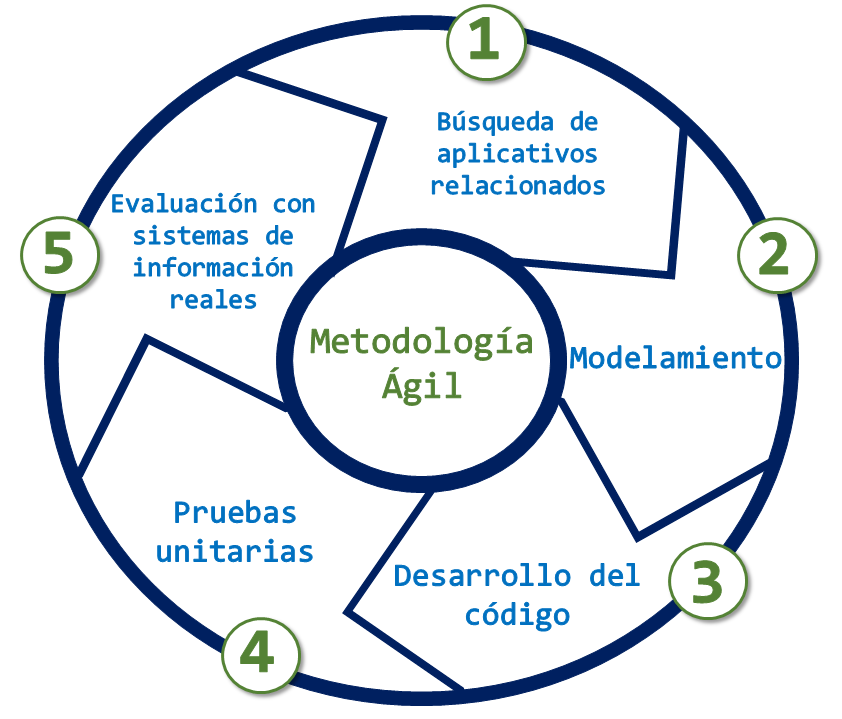
\includegraphics[width=10cm]{images/metodologia.png}
		\caption{Fases de la metodología.}
		\label{fig:metod}
	\end{figure}
	
	\paragraph{Descripción general de la metodología}
	Las principales razones del uso de una metodología ágil es el uso de un ciclo de desarrollo iterativo e incremental para la ejecución de este proyecto son:
	
	\begin{itemize}
		\item Entregas frecuentes y continuas de forma que puede disponer de una funcionalidad básica en un tiempo mínimo y a partir de ahí un incremento y mejora continua del sistema.
		
		\item Previsible inestabilidad de requisitos. Es posible que el sistema incorpora más funcionalidades de las inicialmente identificadas
		
		\item Es posible que durante la ejecución del proyecto se altere el orden en el que se desean recibir los módulos.
	\end{itemize} 
	
	\paragraph{Roles}
	
	El equipo de esta metodología está conformado por 2 roles, Director de proyecto (DP) y el Desarrollador de Sistemas (DS). Todos los miembros de un equipo de desarrollo tienen diferentes roles en la gestión y supervisión de los proyectos. Todos los roles son necesarios para que el proceso funcione eficientemente. 
	
	\begin{itemize}
		\item \textbf{Director de proyecto (DP):} Se encarga de administrar el proceso del proyecto, su planificación, coordinación con el analista y realizar un seguimiento e informes del progreso del proyecto, en términos de calidad, costo y plazos de entrega. El DP es la interfaz principal entre el propietario del producto y el analista de desarrollo de software.
		
		\item \textbf{Desarrollador de Sistemas (DS):} El desarrollador hace el trabajo. Debe tener la capacidad de organizarse y completar una característica centrada en el cliente. Las principales funciones son:
		
		\begin{itemize}
			\item Comprometerse al inicio de cada modulo y desarrollar todas las funcionalidades en el tiempo determinado.
			
			\item Son responsables de entregar un producto a cada término de un modulo.
			
			\item Definir el desarrollo del sistema.
		\end{itemize} 
	\end{itemize}

	\paragraph{Fases}
	
	\begin{enumerate}
		\item \textbf{Búsqueda de aplicativos relacionados:} Buscar aplicativos que realicen procesos similares al que se esta desarrollando. Se deberán especificar varios criterios sobre sus funcionalidades, ventajas y desventajas, vulnerabilidades, versiones, etc. 
		\item \textbf{Modelamiento:} En esta sección se empezaría a realizar el análisis de requisitos funcionales y no funcionales con los que debe contar el producto final.
		\item \textbf{Desarrollo del código:} Se debe empezar con toda la programación del sistema, es decir la escritura de todo el código usando las estructuras necesarios que permitan cumplir con todos los requisitos planteados en la fase anterior. 
		\item \textbf{Pruebas unitarias:} Con todo el desarrollo del producto finalizado, se empieza una fase de pruebas unitarias. Se deben buscar los posibles escenarios a ocurrir al momento de utilizar el sistema,  verificando si la información de entrada y salida es la correcta o incorrecta. 		
		\item \textbf{Evaluación con sistemas de información reales:} Finalmente se pueden utilizar estudios de caso reales que puedan ser aplicados sobre el producto final.
	\end{enumerate}
	
	\subsection{Marco Conceptual}
	En esta sección, se detalla los modelos teóricos, conceptos, argumentos o definiciones que se han desarrollado o investigado en relación con el tema en particular.
	
	\subsubsection{JSON}
	
	Javascript Object Notation (JSON) es un formato ligero de intercambio de datos. Consisten en asociación de nombres y valores. A pesar de ser independiente del lenguaje de programación, es admitido en una gran cantidad de lenguajes de programación. Se basa en un subconjunto del Estándar de lenguaje de programación JavaScript \parencite{JSON}.
	
    \subsubsection{XML}
    
    Es un lenguaje de marcado similar a HTML. Significa Extensible Markup Language y pertenece a la especificación W3C como lenguaje de marcado de propósito general. Esto significa que, a diferencia de otros lenguajes de marcado, XML no está predefinido, por lo que debe definir su propio marcado. El objetivo principal del lenguaje es compartir datos entre diferentes sistemas, como Internet \parencite{XML-based}.
    
    \subsubsection{Compiladores}
    Están diseñados para traducir un fragmento de código escrito en un de lenguaje de programación a lenguaje de máquina que es, el que puede entender la computadora. El compilador analiza el código fuente en busca de errores antes de la traducción. Si se detecta un error, el compilador
    notificar al autor del código para que pueda arreglarlo.. Además, los compiladores modernos o entornos de desarrollo (IDE), puede sugerir soluciones para algunos tipos de errores usando métodos de corrección de errores \parencite{CoEdit}.
    
    \subsubsection{Lenguajes de modelado}
    Representan una serie de requisitos basados en la construcción de elementos visuales para definir estructuras y comportamientos que tendrán los sistemas computarizados. UML (Lenguaje Unificado de Modelado) a través del mecanismo de perfilado, se han basado históricamente en notaciones gráficas. UML mediante el mecanismo de perfiles, maximiza la comprensión humana y facilita la comunicación entre las partes interesadas como son el cliente y desarrollador \parencite{Blended}. 
    
    También existen lenguajes de modelado personalizados para distintas áreas, como por ejemplo en \parencite{Multi-level} proponen un lenguaje de modelado conceptual multinivel al denominan ML2 (Lenguaje de Modelado Multinivel). El lenguaje está orientado al modelado conceptual multinivel (de dominio) y pretende cubrir un amplio conjunto de dominios multiniveles. En el diseño de ML2 sigue un enfoque basado en principios, definiendo su sintaxis abstracta para reflejar una teoría formal para el modelado multinivel que se fue desarrollado previamente.
	
	\section{METODOLOGÍA}
	
	Para el desarrollo del presente proyecto se tomarán en cuenta la ejecución de varias etapas, aplicando el Modelo de Prototipado para desarrollar un prototipo de la aplicación web que utilice el producto final de esta investigación. A continuación, se describe el enfoque metodológico correspondiente a cada una de las fases. 
	
	\subsection{Búsqueda de aplicativos relacionados}
	
	En esta fase se analizaron varias aplicaciones web que cuentan con la funcionalidad de generar diagramas de clases mediante la escritura de texto. Entre las aplicaciones analizadas se encuentran:
	
	\begin{itemize}
		\item \textbf{yuml: }Es una aplicacion web que permite crear diagramas UML mediante la escritura por comandos en texto plano. Se puede destacar que esta herramienta no permite decidir la ubicación o lugar de un elemento grafico ya que busca la mejor distribución según el diagrama generado (https://yuml.me/)
		
		\item \textbf{mermaid: }Es una herramienta de gráficos y diagramas basada en JavaScript que utiliza definiciones de texto inspiradas en Markdown y un renderizador para crear y modificar diagramas complejos. El propósito principal de Mermaid es ayudar a que la documentación se ponga al día con el desarrollo. También se destaca que la aplicación no permite modificar en tiempo real los diagramas generados (https://mermaid.live/).
		
		\item \textbf{ditaa: }Es una pequeña utilidad de línea de comandos escrita en Java, que puede convertir diagramas dibujados con arte ascii ('dibujos' que contienen caracteres que se asemejan a líneas como | / - ), en gráficos de mapa de bits adecuados. También se destaca que la aplicación no permite modificar en tiempo real los diagramas generados (http://ditaa.sourceforge.net/). 
	\end{itemize}
	
	\subsection{Modelamiento}
	
	En esta etapa se pretende modelar la funcionalidad que tendrán todos los métodos y funciones necesarias para identificar cada símbolo y poder interpretar todo el texto para generar la estructura del diagrama de clases.
	Todo el archivo JavaScript estará conformado por estructuras de datos apuntando a la programación orientada a objetos.
	
	\subsection{Desarrollo del código}
	
	La tercera etapa se dedicará al desarrollo de la librería utilizando el lenguaje de programación JavaScript. Todo el código será escrito en un solo archivo con extensión de tipo .js teniendo como ventaja poder ser vinculado dentro de cualquier archivo HTML que dese utilizar los métodos necesarios para obtener la estructura de todo el diagrama de clases en formato JSON.
	
	La estructura podrá ser utilizada por cualquier herramienta de dibujo externa que permita visualizar el diagrama de clases de la forma tradicional con todos sus componentes. A continuación, se enlista los componentes que podrán ser generados por la librería:
	
	\begin{itemize}
		\item Entidades
		\item Interfaces
		\item Enumeradores
		\item Atributos
		\item Métodos
		\item Constructores de clases
		\item Relaciones
	\end{itemize}

	\subsection{Pruebas unitarias}
	En esta fase se pretende realizar todas las pruebas posibles a las funciones que se realizaron en la fase anterior, ingresando algunos textos utilizando los símbolos esperando los valores que devuelva la librería. Algunos de los textos que serán ingresados son los siguientes:
	
	\begin{itemize}
		\item \begin{verbatim}
			Create an user *(user %.username=String, .password=String,
			.status=Status, .user type=UserType, .person=Tutor%) object
		\end{verbatim}
		
		\item \begin{verbatim}
			*(TutorDAO &id=Int [/Save/=Tutor{.tutor=Tutor}])s the tutor 
			data in the database. *¡(TutorDAO)<<*(tutor)¡
		\end{verbatim}
	
		\item \begin{verbatim}
			*(UserDAO &-id=Int [/Save/=User{.user=User}])s the user data 
			in the database. *¡(UserDAO)<<*(User)¡
		\end{verbatim}
	
		\item \begin{verbatim}
			This use case ends when the system displays the *(@Login) 
			login Interface. *¡(Login)<<*(UserDAO)¡
		\end{verbatim}
		
	\end{itemize}
	
	\subsection{Evaluación con sistemas de información reales}
	
	Se utilizaran estudios de caso con sistemas de información reales para crear las descripciones de los casos de uso extendidos de forma natural. Luego se implementaron los símbolos como se crea conveniente, dependiendo de los requisitos ingresados en el texto. Finalmente se utilizara la librería para observar como devuelve el texto nuevamente en forma natural adicional la estructura del diagrama de clases.
	
	\subsection{Modelo de prototipado}
	El Modelo de Prototipado se aplica cuando la información detallada relacionada a requerimientos de entrada y salida del sistema no está disponible. En este modelo se asume que tal vez no todos los requerimientos son conocidos en el inicio del desarrollo del sistema. Se usa generalmente cuando un sistema no existe, o en caso de un largo y complejo sistema, cuando no hay procesos manuales para determinar los requerimientos. Los pasos que se ejecutan en el modelo de prototipado son: 
	
	\begin{enumerate}
		\item \textbf{Obtención y análisis de requisitos:} es el punto de partida del modelo. El usuario es entrevistado para conocer los requisitos del sistema.
		
		\item \textbf{Diseño rápido}: teniendo claro todos los requisitos, se procede a crear un diseño rápido y preliminar incluyendo solo los aspectos más importantes 
		
		\item\textbf{ Construir el prototipo:} se trabaja con la información tomada por el diseño rápido y crear el prototipo de la aplicación.
		
		\item \textbf{Evaluación de usuarios}: el sistema es presentado a varios usuarios para evaluar y verificar sus puntos fuertes y débiles Se reciben comentarios y sugerencias que serán analizadas por los desarrolladores.
		
		\item \textbf{Reajuste del prototipo:} el prototipo actual debe reajustarse según los nuevos requerimientos, es decir que, se debe crear un nuevo prototipo con la información adicional proporcionada por los usuarios evaluados. Este nuevo prototipo será reevaluado justo como el anterior. Este proceso se repite hasta que se cumplan todos los requerimientos especificados por el usuario. Cuando el usuario esté satisfecho con el resultado, se desarrollará un sistema final basado en el prototipo final. 
		
		\item \textbf{Implementación y mantenimiento:} Una vez que se tenga listo el sistema, ya estará listo para ser desplegado a producción. El sistema se somete a un mantenimiento de rutina para minimizar el tiempo de inactividad y evitar fallas a gran escala.
		
	\end{enumerate}
	
	\newpage
	
	\begin{landscape}
	
	\section{CRONOGRAMA DE ACTIVIDADES}
	\begin{figure}[h!]
		\centering
		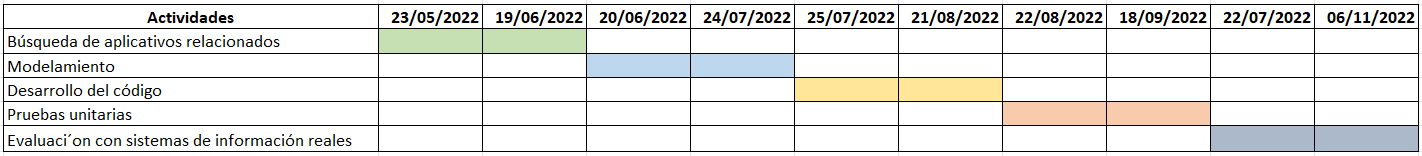
\includegraphics[width=\linewidth]{images/cronograma.png}
		\caption{Cronograma de actividades.}
		\label{fig:usecaseEasyIoT}
	\end{figure}
	
	\end{landscape}
	
	\begin{table}[!ht]
		\centering
		\begin{tabular}{|l|l|l|}
			\hline
			\multicolumn{1}{|c|}{\textbf{Fecha/actividad}}                                                                                                                                                            & \textbf{Inicio}     & \textbf{Finalización} \\ \hline
			\textbf{Búsqueda de aplicativos relacionados}                                                                                                                                                             & \textbf{23-05-2022} & \textbf{19-06-2022}   \\ \hline
			\begin{tabular}[c]{@{}l@{}}Investigar aplicaciones que cuenten con \\ funcionalidades similares al proyecto a desarrollar.\end{tabular}                                                                   & 23-05-2022          & 29-05-2022            \\ \hline
			\begin{tabular}[c]{@{}l@{}}Analizar criterios básicos de las tecnologías \\ encontradas como por ejemplo: (funcionalidades, \\ ventajas y desventajas, vulnerabilidades, \\ versiones, etc.)\end{tabular} & 31-05-2022          & 19-06-2022            \\ \hline
			\textbf{Modelamiento}                                                                                                                                                                                     & \textbf{20-06-2022} & \textbf{24-07-2022}   \\ \hline
			Análisis de los requisitos funcionales                                                                                                                                                                    & 20-06-2022          & 11-07-2022            \\ \hline
			Análisis de los requisitos no funcionales                                                                                                                                                                 & 11-07-2022          & 24-07-2022            \\ \hline
			\textbf{Desarrollo del código}                                                                                                                                                                            & \textbf{25-07-2022} & \textbf{21-08-2022}   \\ \hline
			\begin{tabular}[c]{@{}l@{}}Crear métodos y funciones que verifiquen los \\ símbolos usados por la herramienta TDDT4IoTs\end{tabular}                                                                      & 25-07-2022          & 31-07-2022            \\ \hline
			\begin{tabular}[c]{@{}l@{}}Crear la estructura JSON y XML del diagrama \\ de clases que será retornado como respuesta \\ de la librería\end{tabular}                                                      & 01-08-2022          & 21-08-2022            \\ \hline
			\textbf{Pruebas unitarias}                                                                                                                                                                                & \textbf{22-08-2022} & \textbf{18-09-2022}   \\ \hline
			\begin{tabular}[c]{@{}l@{}}Crear los textos con los símbolos que serán \\ utilizados como textos de entrada\end{tabular}                                                                                  & 22-08-2022          & 31-08-2022            \\ \hline
			\begin{tabular}[c]{@{}l@{}}Comparar la información de respuesta que \\ debió generar la librería con la que genero\end{tabular}                                                                           & 01-09-2022          & 18-09-2022            \\ \hline
			\textbf{Evaluación con sistemas de información reales}                                                                                                                                                    & \textbf{19-09-2022} & \textbf{06-11-2022}   \\ \hline
		\end{tabular}
		\caption{Cronograma detallado por fecha de lo que se pretende realizar.}
		\label{tab:my-table}
	\end{table}
	
	\section{RESULTADOS ESPERADOS}
	
	\begin{itemize}
		
		\item Para poder utilizar la información generada por la librería se organizaran todos los datos obtenidos por el texto ingresando especificando las funcionalidades que tendrá el software mediante las descripciones de los casos de uso extendidos, se utilizaran dos formatos de archivos como lo son: JSON Y XML. Estas estructuras deberán permitir modificar el diagrama de clases con otras librerías de desarrollo para crear diferentes tipos de diagramas como por ejemplo: jsUML, JointJS, Rappid etc. 
		
		\item Diseñar una manera de retroalimentar a los usuarios de TDDT4IoTs mediante mensajes de alerta con diferentes tipos de estado identificados por varios colores. Cada mensaje mencionara los errores detectados en la escritura de los casos de uso.
		
		\item Al momento de contar con todos los objetivos específicos planteados para este proyecto, se realizaran casos de uso sobre sistemas de información demostrando la generación de su respectivo diagrama de clases dependiendo de las descripciones ingresadas por el analista. 
		
	\end{itemize}
	
	\printbibliography[title={\thesection. BIBLIOGRAFÍA}]
	
	\begin{tabular}{@{}p{3in}p{3in}@{}}
		\vspace{3cm} \dotfill   & \vspace{3cm} \dotfill\\
		\vspace{-1cm}
		\begin{center}
			\textbf{Firma de responsabilidad del  Estudiante}
			Carvajal Suárez Dúval Ricardo   \\ 
			\textbf{CC.:} 070638894-9  
		\end{center}   
		& 
		\vspace{-1cm}
		\begin{center}
			\textbf{{ Firma de responsabilidad del  Docente Auspiciante}} \\
			Ing. Gleiston Ciceron Guerrero Ulloa, MDS
			\textbf{CC.:} 091353175-2 
		\end{center}  \\                 
		& \\[8ex]
	\end{tabular}

	
\end{document}